\section{Desarrollo/Análisis}
Gracias a lo consultado en \ref{web3}, fue posible realizar todas las configuraciones necesarias para empezar con el uso del programa \texttt{IMU\_ Capture.ino} disponible en \ref{ArduinoSketches_1}, el cual se encarga de leer la aceleración y el giroscopio de la placa e imprime por un segundo en el monitor serial (por consola del IDE) cuando una velocidad significativa es detectada. Además, es posible activar el \texttt{Serial Plotter} para graficar los datos. Lo anterior se muestra a continuación.

\begin{figure}[H]
   \begin{minipage}{0.48\textwidth}
     \centering
     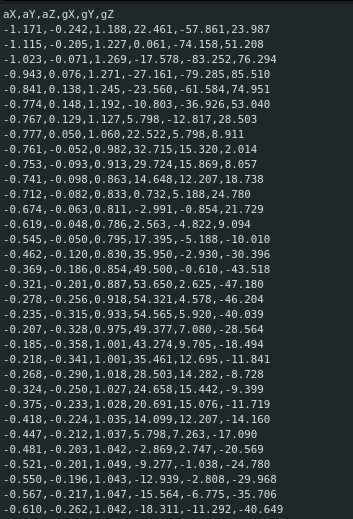
\includegraphics[width=.7\linewidth]{Imagenes/4}
     \caption{ Registro del giroscopio}\label{Fig_4}
   \end{minipage}\hfill
   \begin{minipage}{0.7\textwidth}
     \centering
     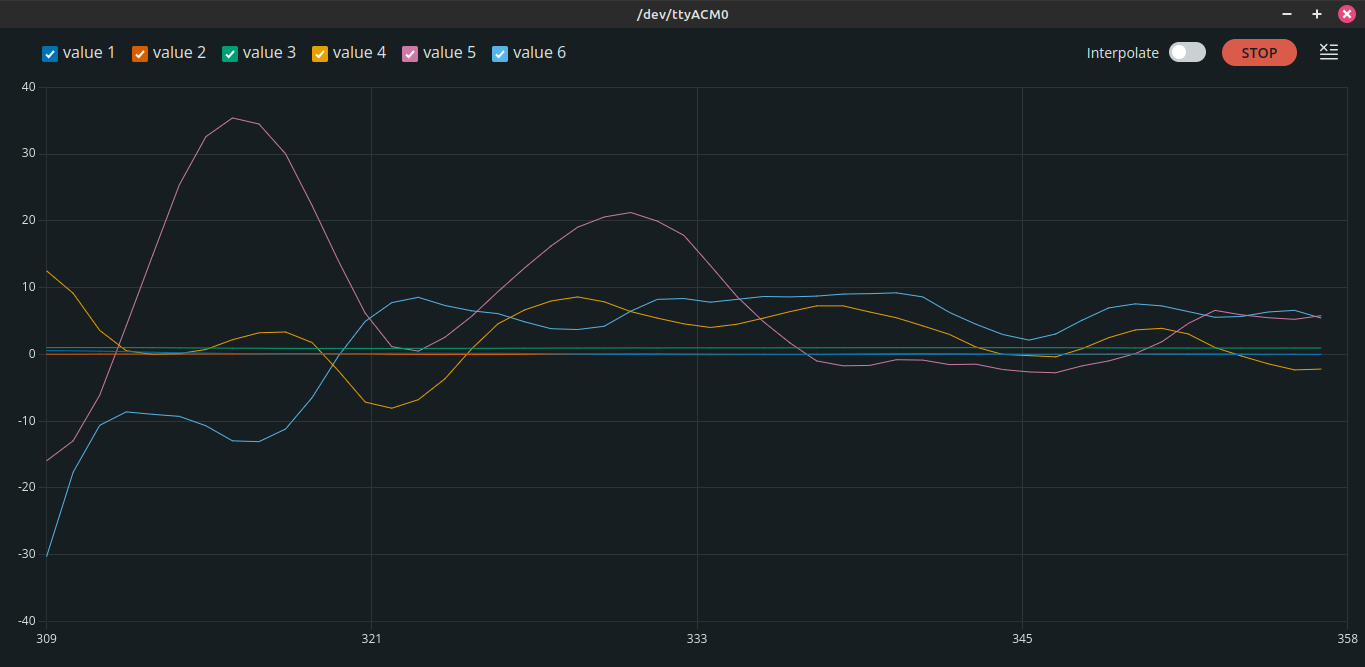
\includegraphics[width=.7\linewidth]{Imagenes/5.png}
     \caption{Graficación del movimiento }\label{Fig_5}
   \end{minipage}
\end{figure}
De la figura \ref{Fig_4}, se tiene las coordenadas que registran el movimiento realizado, que de hecho es un golpe hacia la pantalla de la PC. Luego, en la figura \ref{Fig_5} muestra las ondas del golpe. Hecho esto, se procede a realizar un pequeño script de Python para grabar todos estos datos en un archivo .csv. Por lo que una vez cargado el código \texttt{IMU\_ Capture.ino} se cierra el IDE de Arduino y se ejecuta el script. De donde se realizaron 3 movimientos.
\begin{itemize}
\item Golpe hacia la pantalla (en una sola dirección).
\item Alzar el brazo con diferentes direcciones.
 \item Movimiento circular en contra de las manecillas del reloj.
\end{itemize}
Se tomaron 1750 muestras para los 3 movimientos, un aproximado de \SI{25}{\s} realizando la misma tarea. Ahora, con base a estos datos se realizó el entrenamiento con ayuda de \ref{web4}.

%\begin{figure}[H]
%\centering
%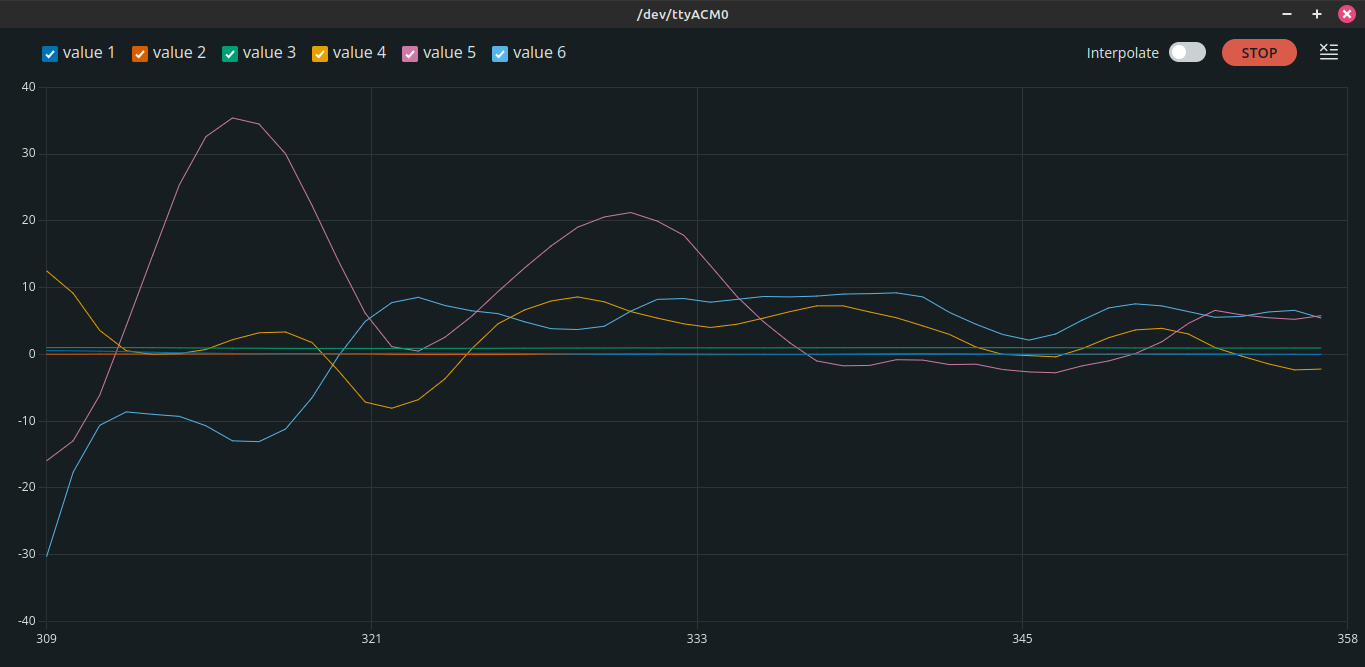
\includegraphics[width=.55\linewidth]{Imagenes/5.png}
% \caption{Funcionamiento del giroscopio.}
% \label{fig_gyro}
%\end{figure}


\newpage